\documentclass[usenames,dvipsnames,10pt]{beamer}

\mode<presentation>
{
\usetheme[width=0.7in]{Hannover}
  \setbeamercovered{invisible}
}
\usepackage{bm} % for some fonts
\usepackage{csquotes} % quotations

\usepackage[english]{babel}
\usepackage[latin1]{inputenc}

\usepackage{times}

\usepackage{hyperref}
\usepackage{booktabs}

\usepackage{takahashi} % for full-page slide

\usepackage{tikz}
\usetikzlibrary{positioning}

\hypersetup{colorlinks=true,
    linkcolor=blue,
    citecolor=blue,
    filecolor=blue,
    urlcolor=blue,
    unicode=false}

\usepackage{amsmath, amsfonts, amssymb, xspace, xcolor, url}

\usepackage{listings}
% \lstset{frame=none, showstringspaces=false, basicstyle=\ttfamily\footnotesize,
%   xleftmargin=-8mm,language=Haskell}
%\lstset{frame=none, showstringspaces=false, 
%  basicstyle=\ttfamily\bfseries\scriptsize,
%  language=Python,breaklines=false,keywordstyle=\bfseries}

\newcommand{\name}[1]{{\color{blue}{#1}}}
\newcommand{\stack}[1]{\begin{tabular}{@{}c@{}}#1\end{tabular}}

\renewcommand{\arraystretch}{1.1} %so that tables with equations do not look crowded

\title{\textbf{Generating Software for Well-Understood Domains}}

%\subtitle
%{Include Only If Paper Has a Subtitle}

\author{\underline{Jacques Carette}, W. Spencer Smith, Jason Balaci}

\institute[McMaster University]
{
  Computing and Software Department\\
  McMaster University
}
% - Keep it simple, no one is interested in your street address.

\date[EVCS 2023] % (optional, should be abbreviation of conference name)
{EVCS 2023}

\subject{research software, software engineering, code generation, domain engineering}
% This is only inserted into the PDF information catalog. Can be left
% out. 

% If you have a file called "university-logo-filename.xxx", where xxx
% is a graphic format that can be processed by latex or pdflatex,
% resp., then you can add a logo as follows:

%\pgfdeclareimage[height=0.5cm]{Mac-logo}{McMasterLogo}
%\logo{\pgfuseimage{Mac-logo}}

% Delete this, if you do not want the table of contents to pop up at
% the beginning of each subsection:
% \AtBeginSubsection[]
% {
%   \begin{frame}<beamer>
%     \frametitle{Outline}
%     \tableofcontents[currentsection,currentsubsection]
%   \end{frame}
% }

% If you wish to uncover everything in a step-wise fashion, uncomment
% the following command: 

%\beamerdefaultoverlayspecification{<+->}

\beamertemplatenavigationsymbolsempty 

\begin{document}

%%%%%%%%%%%%%%%%%%%%%%%%%%%%%%%%%%%%%%
\hoffset=-.4in %removing side bar for these frames
\begin{frame}[plain]

\begin{tikzpicture}[remember picture,overlay]
  \node [xshift=1.3cm,yshift=0cm] at (current page.center)
  {
  
\includegraphics[width=1.5\textwidth]{generate_all_the_things_faint.jpeg}
  };
\end{tikzpicture}

\titlepage

\end{frame}
\hoffset=0in %restore
%%%%%%%%%%%%%%%%%%%%%%%%%%%%%%%%%%%%%%

\begin{frame}

\frametitle{Old Fashioned?}

\blockquote[][\\ \hfill-- \textbf{Referee 2}]{
\small{
I enjoyed reading this short paper. It is a very classical paper, reminiscing
of the DSL systems of the early days, like Neighbor's 
\name{Draco} and Baxter's \name{DMS}.
Indeed, it is an old vision to represent domain knowledge first-class, to avoid
duplication, and offer variation points to make engineering trade-offs.}
}

\vspace*{5mm}
\blockquote[][\hfill -- \textbf{Referee 3}]{
\small{
As general feedback, the paper's message reads a bit ``old-fashioned''. The
``well-understood'' qualification is nice (because it qualifies what would
otherwise be overly-general statements) but the actual benefit claimed is
straight out of the playbook of the "automatic programming" community of the
80s and 90s. For instance, I was strongly reminded of Novak's 
\name{GLisp}...}
}

% Add pic from Draco and GLisp paper?
\end{frame}

%%%%%%%%%%%%%%%%%%%%%%%%%%%%%%%%%%%%%%
\begin{frame}
  
  \frametitle{Well Understood?}
  
  Given $F, Q, \kappa, \phi, \gamma$ calculate:

  \begin{equation} \label{EqImplicitFEM}
    \mathbf{K} = \int_V \mathbf{B}^T \mathbf{D}^{vp} \mathbf{B} dV; \mathbf{F} = \mathbf{R}_i - \int_V \mathbf{B}^T \bm{\sigma}_i dV + \int_V \mathbf{B}^T
    \Delta
    \bm{\sigma}^{vp} dV
    \end{equation}
    with
    \begin{equation}
    \mathbf{D}_{vp} =
    \mathbf{D} \left [
    \mathbf{I} - {\Delta t} C_1 \lambda' \frac{\partial Q}{\partial \bm{\sigma}} \left ( \frac{\partial F}{\partial
    \bm{\sigma}} \right )^{T} \mathbf{D}
    \right ], \lambda' = \frac{d \lambda}{d F}
    \end{equation}
    \begin{equation}
    \Delta \bm{\sigma}^{vp} = \Delta t C_1 \lambda \mathbf{D} \frac{\partial Q}{\partial \bm{\sigma}}
    \end{equation}
    \begin{equation}
    C_1 = [1 + \lambda' {\Delta t} (H_e + H_p)]^{-1}
    \end{equation}
    \begin{equation}
    \label{HEE}
    H_e = \left ( \frac{\partial F}{\partial \bm{\sigma}} \right )^T \mathbf{D} (\frac{\partial Q}{\partial \bm{\sigma}})
    \end{equation}
    \begin{equation}
    H_p = -\frac{\partial F}{\partial \kappa} \left ( \frac{\partial \kappa}{\partial \bm{\epsilon}^{vp}}
    \right )^T \frac{\partial Q}{\partial \bm{\sigma}}
    \end{equation}
    %where $\mathbf{I}$ is the identity matrix.
  
\end{frame}
  
%%%%%%%%%%%%%%%%%%%%%%%%%%%%%%%%%%%%%%
%\begin{frame}
%Well Understood
%\end{frame}
%\hoffset=-.4in %removing side bar for these frames    
{\setbeamercolor{background canvas}{bg=black}
\addtolength\textwidth{-.4in} 
\setlength\hsize{\textwidth} 
\setlength\columnwidth{\textwidth}
\takahashi{\color{yellow}{\stack{Well\\Understood!}}}
}
%\hoffset=0in %restore  
  
%%%%%%%%%%%%%%%%%%%%%%%%%%%%%%%%%%%%%%
\hoffset=-.4in %removing side bar for these frames    
\begin{frame}[plain] % knowledge duplication

  \begin{tikzpicture}[remember picture,overlay]
    \node [xshift=0.8cm,yshift=0.0cm] at (current page.center)
    {
    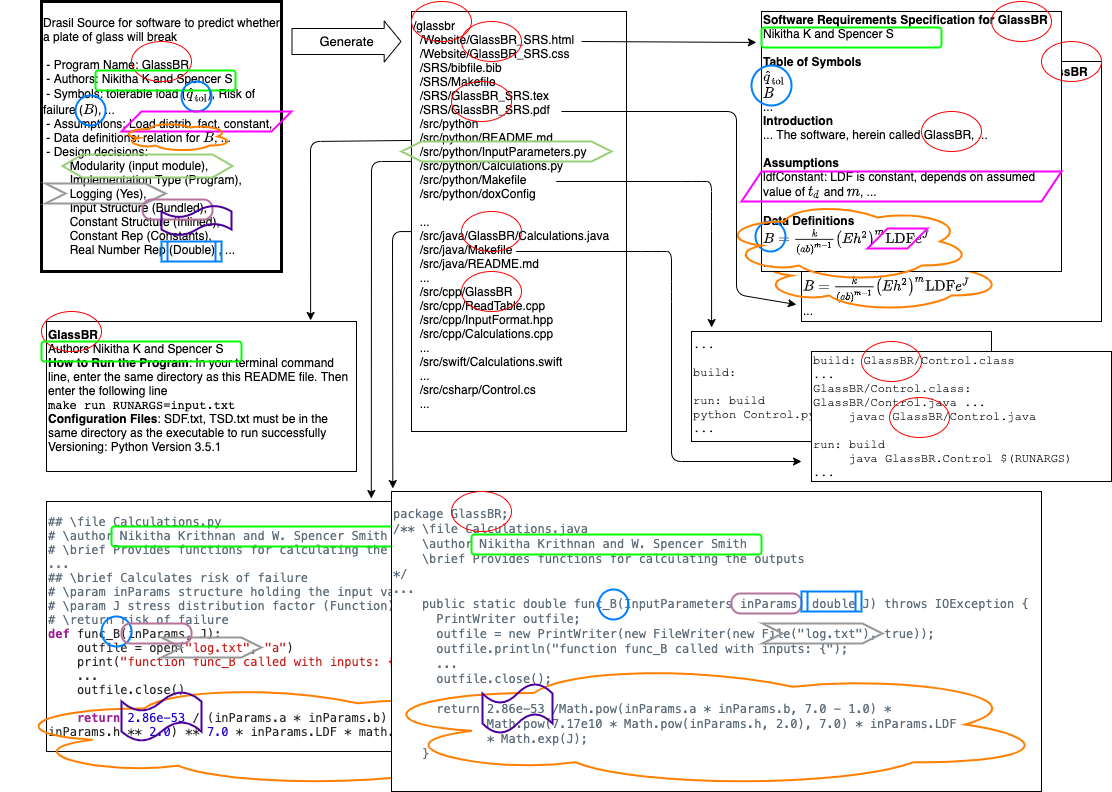
\includegraphics[width=1.2\textwidth]{DrasilSupportsChange.png}
    };
  \end{tikzpicture}
  
\end{frame}
\hoffset=0in %restore  

% redundancy
% recipes for softifacts
% language of design emerges

%%%%%%%%%%%%%%%%%%%%%%%%%%%%%%%%%%%%%%
\begin{frame}
  
  \frametitle{Process}
  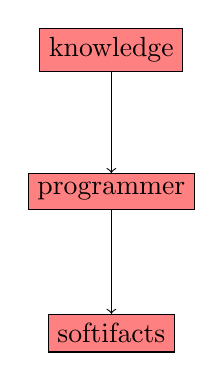
\begin{tikzpicture}[node distance=1.8cm]
    \tikzstyle{every node}=[draw=black,rectangle,fill=red!50];
    \node (A) {knowledge};
    \node (B) [below of=A] {programmer};
    \node (C) [below of=B] {softifacts};

    \draw[->] (A) -- (B);
    \draw[->] (B) -- (C);
  \end{tikzpicture}
  \pause
  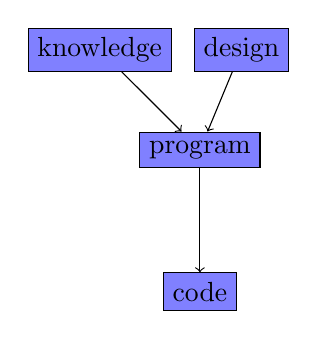
\begin{tikzpicture}[node distance=1.8cm]
    \tikzstyle{every node}=[draw=black,rectangle,fill=blue!50];
    \node (A) {knowledge};
    \node (D) [right of=A] {design};
    \node (B) [below right of=A] {program};
    \node (C) [below of=B] {code};
    \draw[->] (A) -- (B) ;
    \draw[->] (D) -- (B) ;
    \draw[->] (B) -- (C) ;
  \end{tikzpicture}
  \pause
  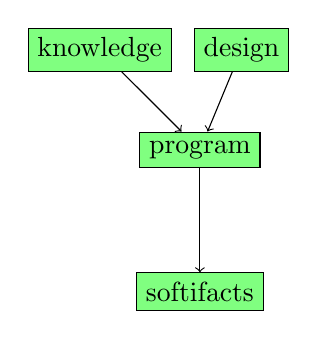
\begin{tikzpicture}[node distance=1.8cm]
    \tikzstyle{every node}=[draw=black,rectangle,fill=green!50];
    \node (A) {knowledge};
    \node (D) [right of=A] {design};
    \node (B) [below right of=A] {program};
    \node (C) [below of=B] {softifacts};
    \draw[->] (A) -- (B);
    \draw[->] (D) -- (B);
    \draw[->] (B) -- (C);
  \end{tikzpicture}
%  - (human-provided) knowledge -> programmer's brains -> softifacts
%  - knowledge + (hp) design -> program -> code
%  - knowledge + (hp) design -> program -> softifacts

\end{frame}
  
%%%%%%%%%%%%%%%%%%%%%%%%%%%%%%%%%%%%%%
\begin{frame}[fragile]
  
  \frametitle{Key Philosophical Differences}
\begin{minipage}{0.48\textwidth}
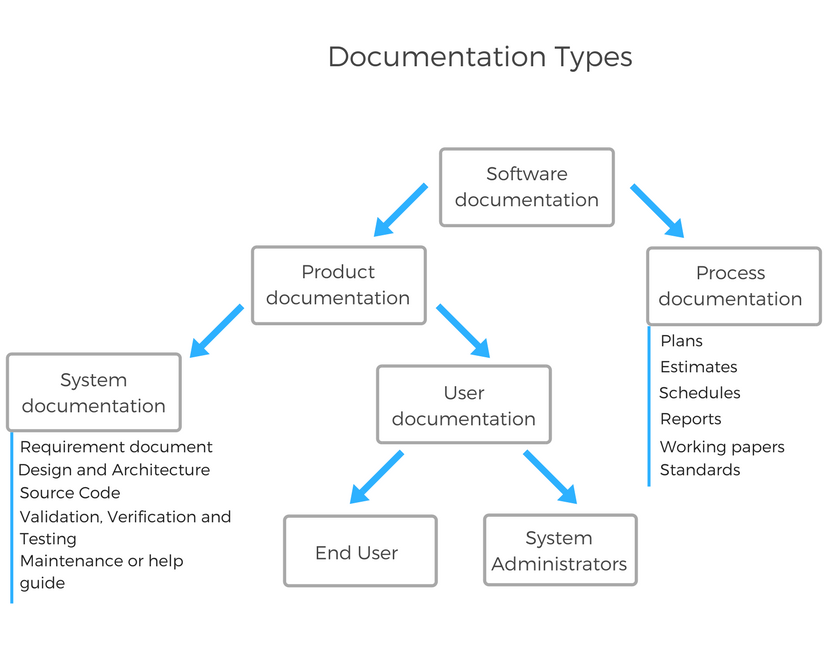
\includegraphics[width=1.0\textwidth]{DocKinds.png}
\end{minipage}
\begin{minipage}{0.48\textwidth}

\includegraphics[width=1.0\textwidth]{BoredAtWork.jpg}
\end{minipage}

\begin{lstlisting}[language=Python,basicstyle=\ttfamily\tiny,
  keywordstyle=\bfseries,breaklines=false]
## \file Projectile.py
# \author Samuel J. Crawford, Brooks MacLachlan, and W. Spencer Smith
# \brief Contains the entire Projectile program
import math
import sys

## \brief Calculates flight duration: the time when the projectile lands (s)
# \param v_launch launch speed: the initial speed of the projectile when launched (m/s)
# \param theta launch angle: the angle between the launcher and a straight line from the launcher to the target (rad)
# \param g_vect gravitational acceleration (m/s^2)
# \return flight duration: the time when the projectile lands (s)
def func_t_flight(v_launch, theta, g_vect):
    return 2.0 * v_launch * math.sin(theta) / g_vect

\end{lstlisting}
\end{frame}
  
%%%%%%%%%%%%%%%%%%%%%%%%%%%%%%%%%%%%%%
\begin{frame}
  
  \frametitle{Better Technology \& Theory}
  \tikzstyle{tech}=[fill=green!60, text=black, circle, draw=green, thick, minimum size=6mm]
  \tikzstyle{techme}=[fill=ForestGreen!60, text=black, circle, draw=green, thick, minimum size=6mm]
  \tikzstyle{theory}=[fill=purple!50, text=black, rectangle, draw=purple, thick, minimum size=6mm]
  \tikzstyle{theoryme}=[fill=purple!80, text=black, rectangle, draw=purple, thick, minimum size=6mm]
   \begin{tikzpicture}[node distance=2cm]
     \node[tech] (Haskell) {Haskell};
     \node[tech] (DSLs) [right of=Haskell] {DSLs};
     \node[techme] (GOOL) [right of=DSLs] {GOOL};
     \node[tech] (PE) [right of=GOOL] {PE};
     \node[techme] (tagless) [right of=PE] {tagless};

     \node[theory] (type) [below of=Haskell] {Type Theory};
     \node[theory] (cat) [below of=GOOL] {Category Theory};
     \node[theoryme] (biform) [below of=tagless] {Biform Theories};
     \node[theory] (lens) [below of=cat] {Lenses};
    \end{tikzpicture}

% Type Theory, Category Theory, Lenses, Biform theories

\end{frame}
  
%%%%%%%%%%%%%%%%%%%%%%%%%%%%%%%%%%%%%%
\hoffset=-.4in %removing side bar for these frames
\begin{frame}[plain]

\vspace*{8mm}
\begin{tikzpicture}[remember picture,overlay]
  \node [xshift=1.3cm,yshift=0cm] at (current page.center)
  {
  
\includegraphics[width=1.5\textwidth]{generate_all_the_things_faint.jpeg}
  };
\end{tikzpicture}

\begin{center}
\color{Blue}{\huge \textbf{What if we generated it \textcolor{Red}{all}$^{*}$?}}
\end{center}

\hspace*{1cm}
\includegraphics[width=0.25\textwidth]{Icon.png}

\hspace*{1.7cm}{\textbf{Drasil}}

\vspace*{1.6cm}
{\scriptsize $^{*}$ when it makes sense do to so}
\end{frame}
\hoffset=0in %restore
\end{document}
